%%
%% Chapter: 6
%%
\cleardoublepage  %  flush all material and start a new page, start new odd numbered page. 
\addchap{Appendices}		%% Add chapter without number
\label{cha:Appendices}      %% No special characters, no space 

\emph{This section contains all
	\begin{itemize}
		\item questionnaires,
		\item interview transcripts,
		\item pilot reports,
		\item detailed tables, etc.
	\end{itemize}
	This section should contain material that supplements the main text of the report (spreadsheets, detailed experimental results, details of equation derivation, program listings, etc.). 
	If an equation is included in the body of the report, the derivation of that equation could be shown in the Appendix, or if you have a graph from a spreadsheet or program calculation, you could include the spreadsheet data or a program listing in the Appendix. 
	The key point is that the Appendix is supplemental information. 
	Depending on what was requested in the problem statement, detailed drawings might also go in the Appendix and only the overall assembly drawing would go in the body.
}

\section*{Appendix I: Work plan}
\addcontentsline{toc}{section}{Appendix I: Work plan}%

\begin{ganttchart}[
	hgrid,
	%vgrid,
	expand chart=\textwidth,  % shrink/expand chart to available width
	milestone/.append style={inner ysep=3mm},  % make milestones more visible
	bar/.append style={fill=red!50}, % make bars red
	%link mid=1, link bulge=1,
	%link/.style={-to, rounded corners = 3pt},
	%link tolerance=0,
	calendar week text={W\currentweek}, % Change from 'Week 5' to 'W5'
	time slot format=isodate
	]{2021-02-01}{2021-04-30}
	%\gantttitlecalendar{year, month=shortname, week=5} \\  % Set week=5 if chart start at week 5
	\gantttitlecalendar{year, month=shortname} \\ % no week shown
	\ganttbar{Task 1}{2021-02-15}{2021-02-20} \\   % One week for Task 1
	\ganttlinkedbar{Task 2}{2021-02-22}{2021-03-06} \\   % two week for Task 2
	\ganttlinkedbar{Task 3}{2021-03-08}{2021-03-27} \\   % three week for Task 3
	\ganttlinkedbar{Task 4}{2021-03-29}{2021-04-03} \\   % One week for Task 4
	\ganttlinkedmilestone{Milestone 1}{2021-04-05}
\end{ganttchart}

\cleardoublepage  % have next section on new odd numbered page (right)
\section*{Appendix II: Budget}
\addcontentsline{toc}{section}{Appendix II: Budget}%

\begin{table}[!h]
	\begin{center}
		\caption{\label{tbl:Budget}Proposed budget}
		\begin{tabular}{llccrr}
			\hline \\
				Item & Description    & Unit      & Quantity  & Rate (Shs.) & Amount (Shs.)    \\
			\\
			\hline \\				
				1    & Food           &           & 2         & 10,000      & 20,000           \\
				2    & Drinks         &           & 2         & 1,000       & 2,000            \\
				3    & Ghost writer   &           & 1         & 478,000     & 478,000          \\
			\\
				& \textbf{TOTAL} & \textbf{} & \textbf{} & \textbf{}   & \textbf{500,000}		\\
			\hline \\ 
		\end{tabular}
	\end{center}
\end{table}

\cleardoublepage  % have next section on new odd numbered page (right)
\section*{Appendix III: Questionnaire}
\addcontentsline{toc}{section}{Appendix III: Questionnaire}%

\centering
\fbox{
	\label{fig:Questionnaire}
	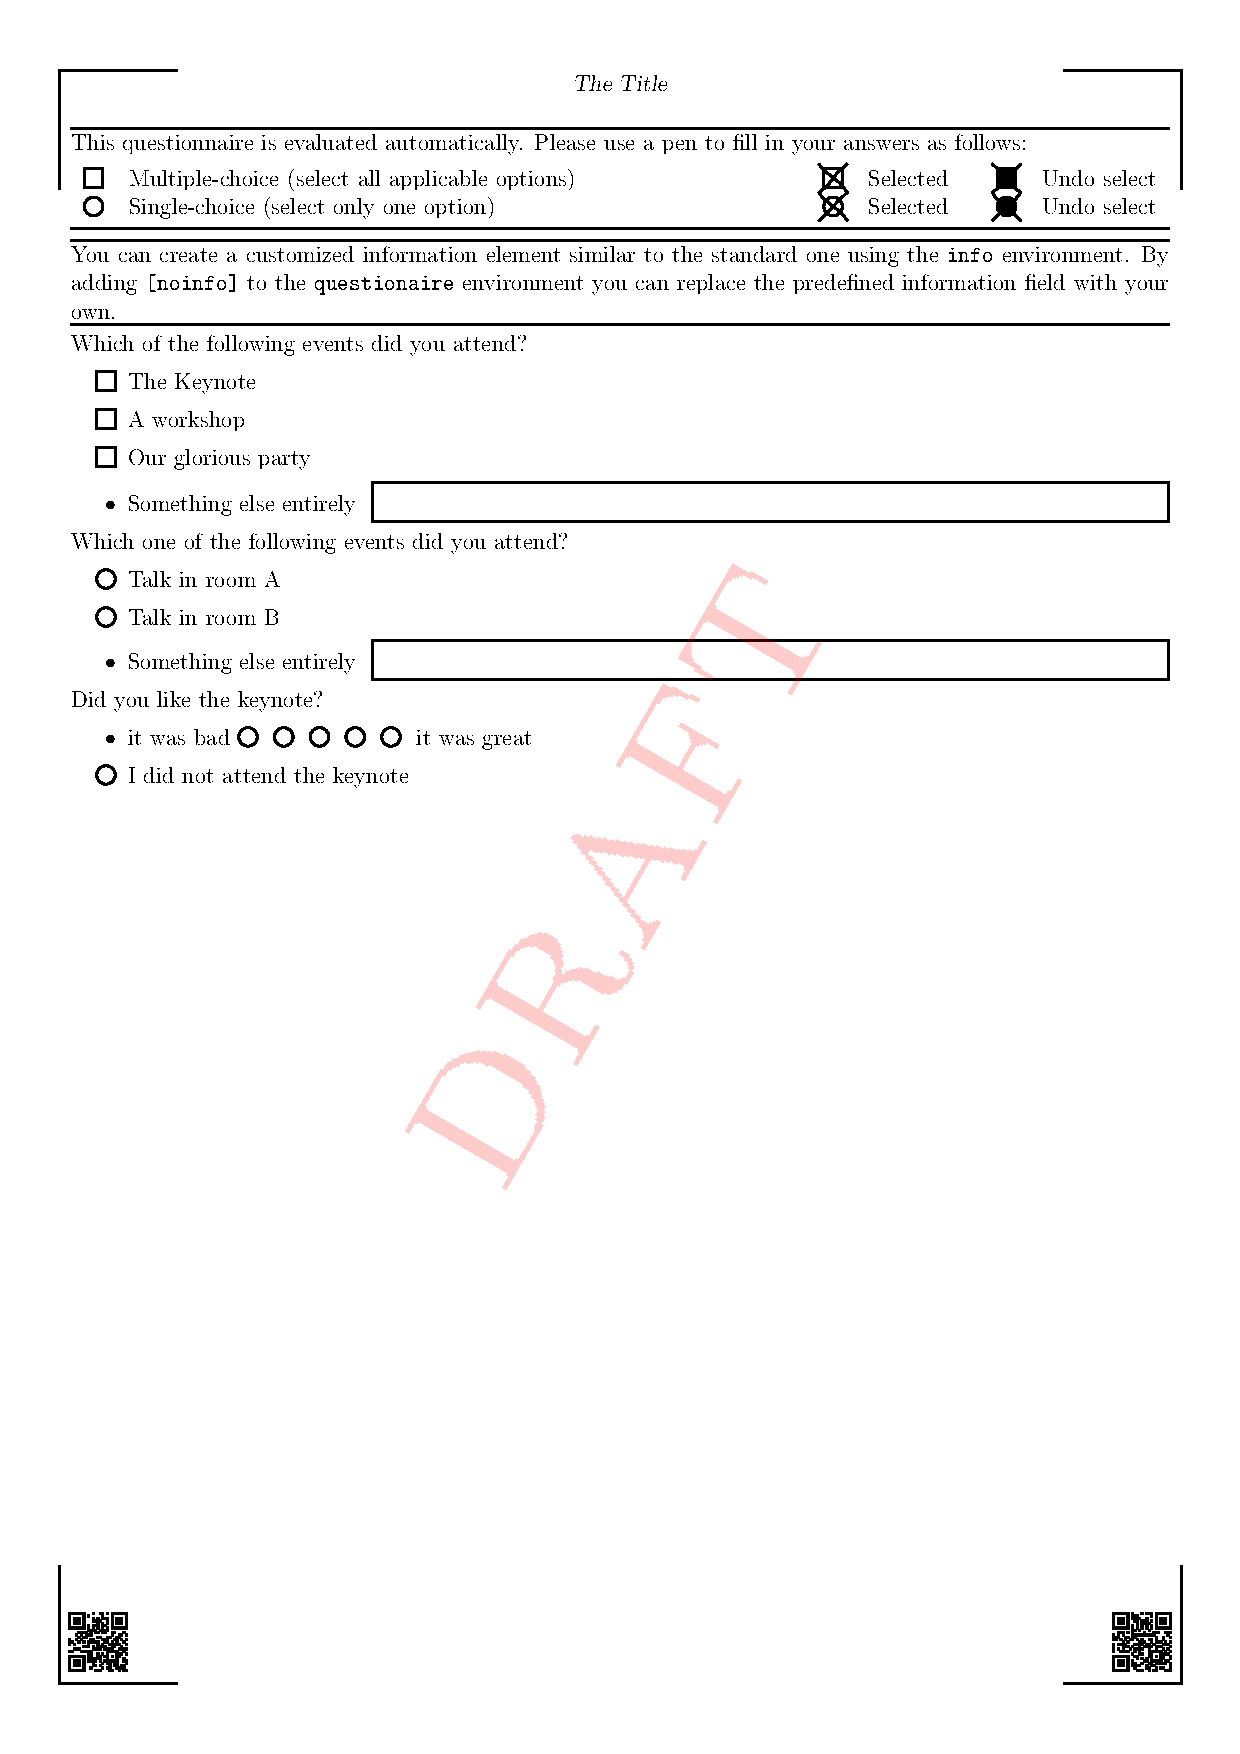
\includegraphics[scale=0.68]{600-Appendices/Questionnaire/Questionnaire}
	%\caption{Questionnaire}
}

\clearpage  % have next section on separate page
\section*{Appendix IV: Some \LaTeX{} examples}

This section is to be deleted/commented by the author.
\paragraph{Demonstration of abbreviations}
Define a glossary entry in file \textit{Acronyms.tex}:
\newline
\verb!\newacronym{utc}{UTC}{Coordinated Universal Time}!
\newline
Use a glossary entry: \verb! \gls{utc} !
\newline
This \LaTeX code \\

\verb*|\gls{utc} is 3 hours behind \gls{adt}.| \\

will produce this: \\

\gls{utc} is 3 hours behind \gls{adt}.\\

At the first time usage, the abbreviation is mentioned in brackets.

With the second usage of an abbreviation, the abbreviated term itself is not shown any more:
\gls{utc} is still 3 hours behind \gls{adt}.\\

\paragraph{Demonstration of a horizontal bar chart}
Fig. \ref{fig:XBarChart} shows an example of a horizontal bar chart generated with tikzpicture (pgfplots package).

\begin{figure}[!h]
	\centering
	\begin{tikzpicture}
		\begin{axis}[xbar,tick align=outside,
			%width=11cm,
			%height=8cm,
			bar width={10pt},
			enlarge y limits=0.13,
			enlarge x limits=false,
			nodes near coords,
			nodes near coords align=horizontal,
			use units,
			xmin=0,
			xmax=60,
			xtick={0,10,...,60},
			x unit=\%,
			xlabel=Reduction in diarrhoea morbidity,
			ytick={1,...,6},
			yticklabels={Hand Washing With Soap, Point-of-use Water Treatment, Sanitation, Hygiene Education, Water Supply, Source Water Treatment}
			]
			\addplot
			[draw=blue,fill=blue!15]
			coordinates
			{(11,1) (25,2) (28,3) (32,4) (39,5) (44,6)};
		\end{axis}
	\end{tikzpicture}
	\caption{\label{fig:XBarChart}Title to a x-bar chart}
\end{figure}

\paragraph{Demonstration of a vertical bar chart}
Fig. \ref{fig:YBarChart} shows an example of a vertical bar chart generated with tikzpicture (pgfplots package).


\begin{figure}
	\centering
	\begin{tikzpicture}
		\begin{axis}[ybar,tick align=outside,
			%width=11cm,
			%height=8cm,
			bar width={10pt},
			enlarge x limits=0.13,
			enlarge y limits=false,
			nodes near coords,
			nodes near coords align=vertical,
			use units,
			ymin=0,
			ymax=100,
			ytick={0,10,...,100},
			y unit=\%,
			ylabel=Response,
			xtick={1,...,7},
			xticklabels={Water for handwashing, Soap for handwashing, Covered pit latrines, Latrines condusive for use, Latrine have doors, Seperate for both boys and girls, Seperate for teachers/pupils},
			x tick label style={rotate=45,anchor=east}
			]
			\addplot
			[draw=blue,fill=blue!15]
			coordinates
			{(1,25) (2,10) (3,5) (4,45) (5,25) (6,100) (7,100)};
		\end{axis}
	\end{tikzpicture}
	\caption{\label{fig:YBarChart}Title to a y-bar chart}
\end{figure}

\paragraph{Demonstration of a stacked bar chart}
Fig. \ref{fig:StackedBarChart} shows an example of a stacked bar chart generated with tikzpicture (pgfplots package).

\begin{figure}
	\centering
	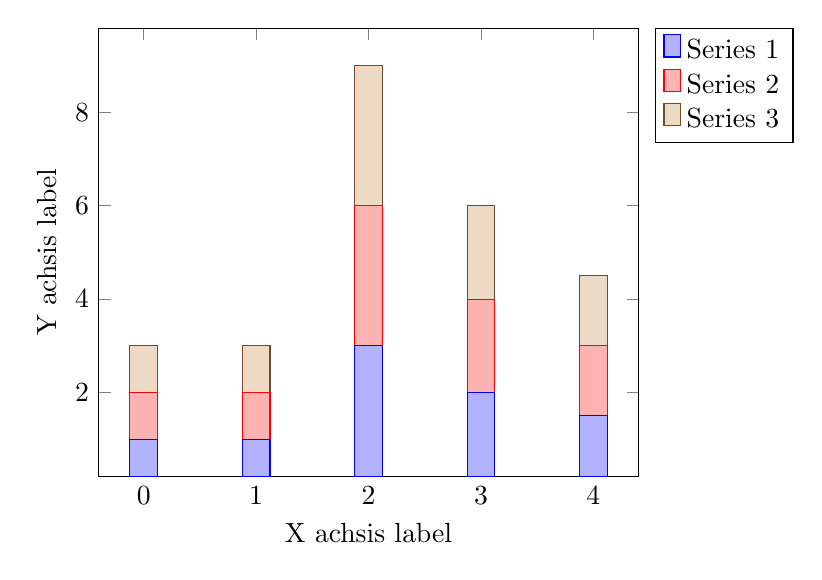
\begin{tikzpicture}
		\begin{axis}[ybar stacked, 
			xlabel=X achsis label, 
			ylabel=Y achsis label,
			legend cell align=left,
			legend pos=outer north east]
			\addplot coordinates 
			{(0,1) (1,1) (2,3) (3,2) (4,1.5)};
			\addplot coordinates
			{(0,1) (1,1) (2,3) (3,2) (4,1.5)};
			\addplot coordinates
			{(0,1) (1,1) (2,3) (3,2) (4,1.5)};
			\legend{Series 1, Series 2, Series 3}
		\end{axis}
	\end{tikzpicture}
	\caption{\label{fig:StackedBarChart}Title to a stacked bar chart}
\end{figure}

\paragraph{Demonstration of a clustered bar chart}
Fig. \ref{fig:ClusteredBarChart} shows an example of a clustered bar chart generated with tikzpicture (pgfplots package).

\begin{figure}
	\centering
	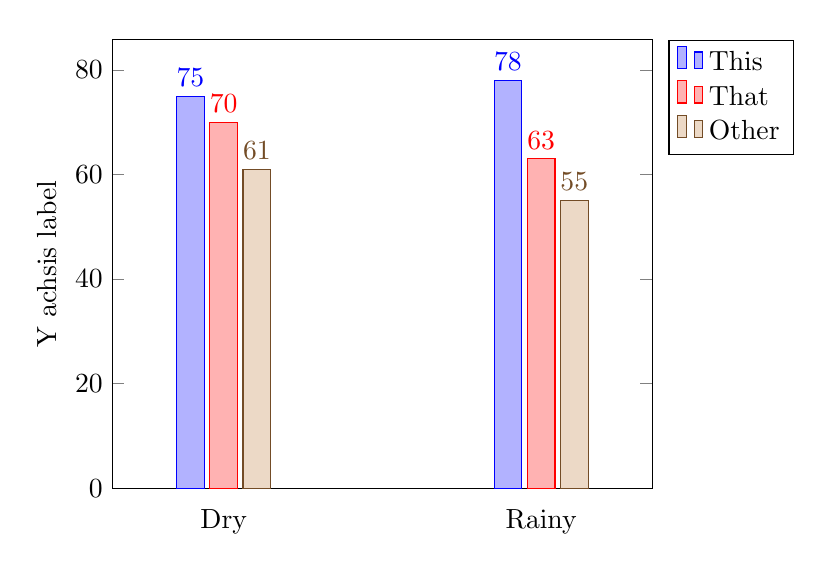
\begin{tikzpicture}
		\begin{axis}  
			[  
			ybar,
			ylabel={Y achsis label}, % there should be no line gap between the rows here. Otherwise, latex will show an error.  
			symbolic x coords={Dry, Rainy},  
			xtick=data,  % groups plots around same tick
			enlarge x limits=0.35, % increases the axis range by 25%
			ymin=0,
			major x tick style = transparent,
			nodes near coords,  
			nodes near coords align={vertical},
			legend cell align=left,
			legend pos=outer north east
			]  
			\addplot coordinates {(Dry, 75) (Rainy, 78)}; % these are the measures of a particular bar graph. The tick marks of the y-axis will be adjusted automatically according to the data values entered in the coordinates.  
			\addplot coordinates {(Dry, 70) (Rainy, 63)};  
			\addplot coordinates {(Dry, 61) (Rainy, 55)};  
			\legend{This, That, Other}  
			
		\end{axis} 
	\end{tikzpicture}
	\caption{\label{fig:ClusteredBarChart}Title to a clustered bar chart}
\end{figure}

\paragraph{Demonstration of a pie chart}
Fig. \ref{fig:PieChart} shows an example of a pie chart generated with tikzpicture (pgf-pie package).

\begin{figure}
	\centering
	\begin{tikzpicture}
		\pie [rotate = 180]
		{
			62/Category A,
			32/Category B, 
			6/Other
		}
		\end{tikzpicture}
	\caption{\label{fig:PieChart}Title to the pie chart}
\end{figure}

\paragraph{Demonstration of a line chart}
Fig. \ref{fig:LineChart} shows an example of a simple chart generated with tikzpicture (packages pgfplots and pgfplotstable). 
The regression is also rendered and the formula $ y(x_i) = a \cdot x_i + b$ displayed. The values a and b will be stored globally.

\begin{figure}
	\centering
	\begin{tikzpicture}
		\begin{axis}[legend pos=outer north east]
			\addplot table[row sep=\\] {% plot X versus Y. This is original data.
				X Y\\
				1 1 \\
				2 4\\
				3 9\\
				4 16\\
				5 25\\
				6 36\\
			};
			\addplot table[row sep=\\,
			y={create col/linear regression={y=Y}}] % compute a linear regression from the input table
			{
				X Y\\
				1 1 \\
				2 4\\
				3 9\\
				4 16\\
				5 25\\
				6 36\\
			};
			\addlegendentry{$y(x)$}
			\addlegendentry{%
				$\pgfmathprintnumber{\pgfplotstableregressiona} \cdot x
				\pgfmathprintnumber[print sign]{\pgfplotstableregressionb}$}
		\end{axis}

	\end{tikzpicture}
	\caption{\label{fig:LineChart}Title to the line chart}
\end{figure}

\paragraph{Demonstration of a table}
Table \ref{tbl:Salinity-EC} shows an example of a table. Different parts of the Final Year Report and their corresponding weights for marking them can be viewed at table \ref{tbl:ModuleWeight}.\\
A help to generate LaTeX tables can be found at \url{https://www.tablesgenerator.com/}.
\begin{table}
	\begin{center}
		\caption{\label{tbl:Salinity-EC}Conductivity values measured for defined salinity values}
		\begin{tabular}{cc}
			\hline \\
			Salinity [g/L]	& 	Electrical Conductivity [mS/cm]\\    
			\\
			\hline \\
			40	&	63,3	\\
			35	&	55,1	\\
			30	&	47,2	\\
			25	&	40,4	\\
			20	&	32,9	\\
			15	&	25,5	\\
			10	&	17,53	\\
			5	&	9,39	\\
			\hline \\
		\end{tabular}  
	\end{center}
\end{table}

\begin{table}
	\begin{center}
		\caption{\label{tbl:ModuleWeight}Module CIV4202 Final Year Report - Assessment}
		\begin{tabular}{llc}
			\hline \\
			Category					& Chapter or Feature				& Weight \\
			\\
			\hline \\
			Engineering Content (60\%)	& Introduction and Objectives		& 10\%   \\
										& Problem definition				& 5\%    \\
										& Literature review					& 5\%    \\
										& Methods							& 15\%   \\
										& Results and Discussion			& 15\%   \\
										& Conclusions and recommendations	& 10\%   \\
			Language (25\%)				& Grammar and spelling				& 15\%   \\
										& Sentence structure				& 10\%   \\
			References (15\%)			& Use of references					& 10\%   \\
										& Quality and format of references	& 5\%    \\
			\hline \\
		\end{tabular}
	\end{center}
\end{table}

\paragraph{Demonstration of including a PDF}
Fig. \ref{fig:GF543kv} shows an example of a PDF. The section displayed is of a particular page from the PDF and is cropped in size.
\begin{figure}
	\centering
	\includegraphics[height=0.7\textwidth,page=6, trim = 25mm 172mm 25mm 45mm, clip]{600-Appendices/Examples/Datasheet_GF_543}
	\caption{GF ball valve 543 kv-characteristic}
	\label{fig:GF543kv}
\end{figure}

\paragraph{Demonstration of including a graphics}
Fig. \ref{fig:ndulogo} shows an image stored as jpg-file. The file is limited to the page width and is rotated by 90\textdegree. Because of the rotation 'height' becomes 'width'.

\begin{figure}
	\centering
	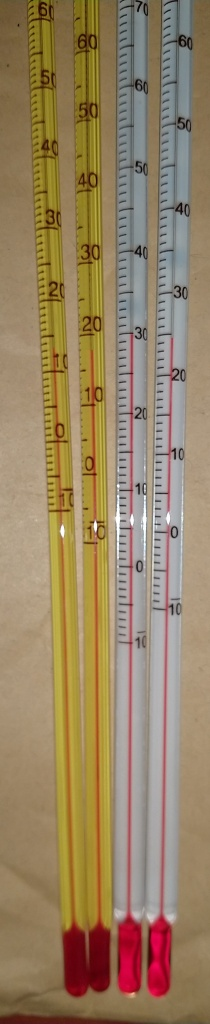
\includegraphics[height=1\textwidth, angle=90]{600-Appendices/Examples/Thermometer.jpg}
	\caption{Thermometers showing different temperature readings.}
	\label{fig:ndulogo}
\end{figure}

\paragraph{Demonstration of including a JPG with labels}
Fig. \ref{fig:HeatExchanger} shows an example of a JPG that has some labels applied.

\begin{figure}
	\centering
	\setlength {\unitlength}{0.1\textwidth}
	\begin{picture} (10,7)(0,0)
		\setlength\fboxsep{1 mm}
		\put(0,0){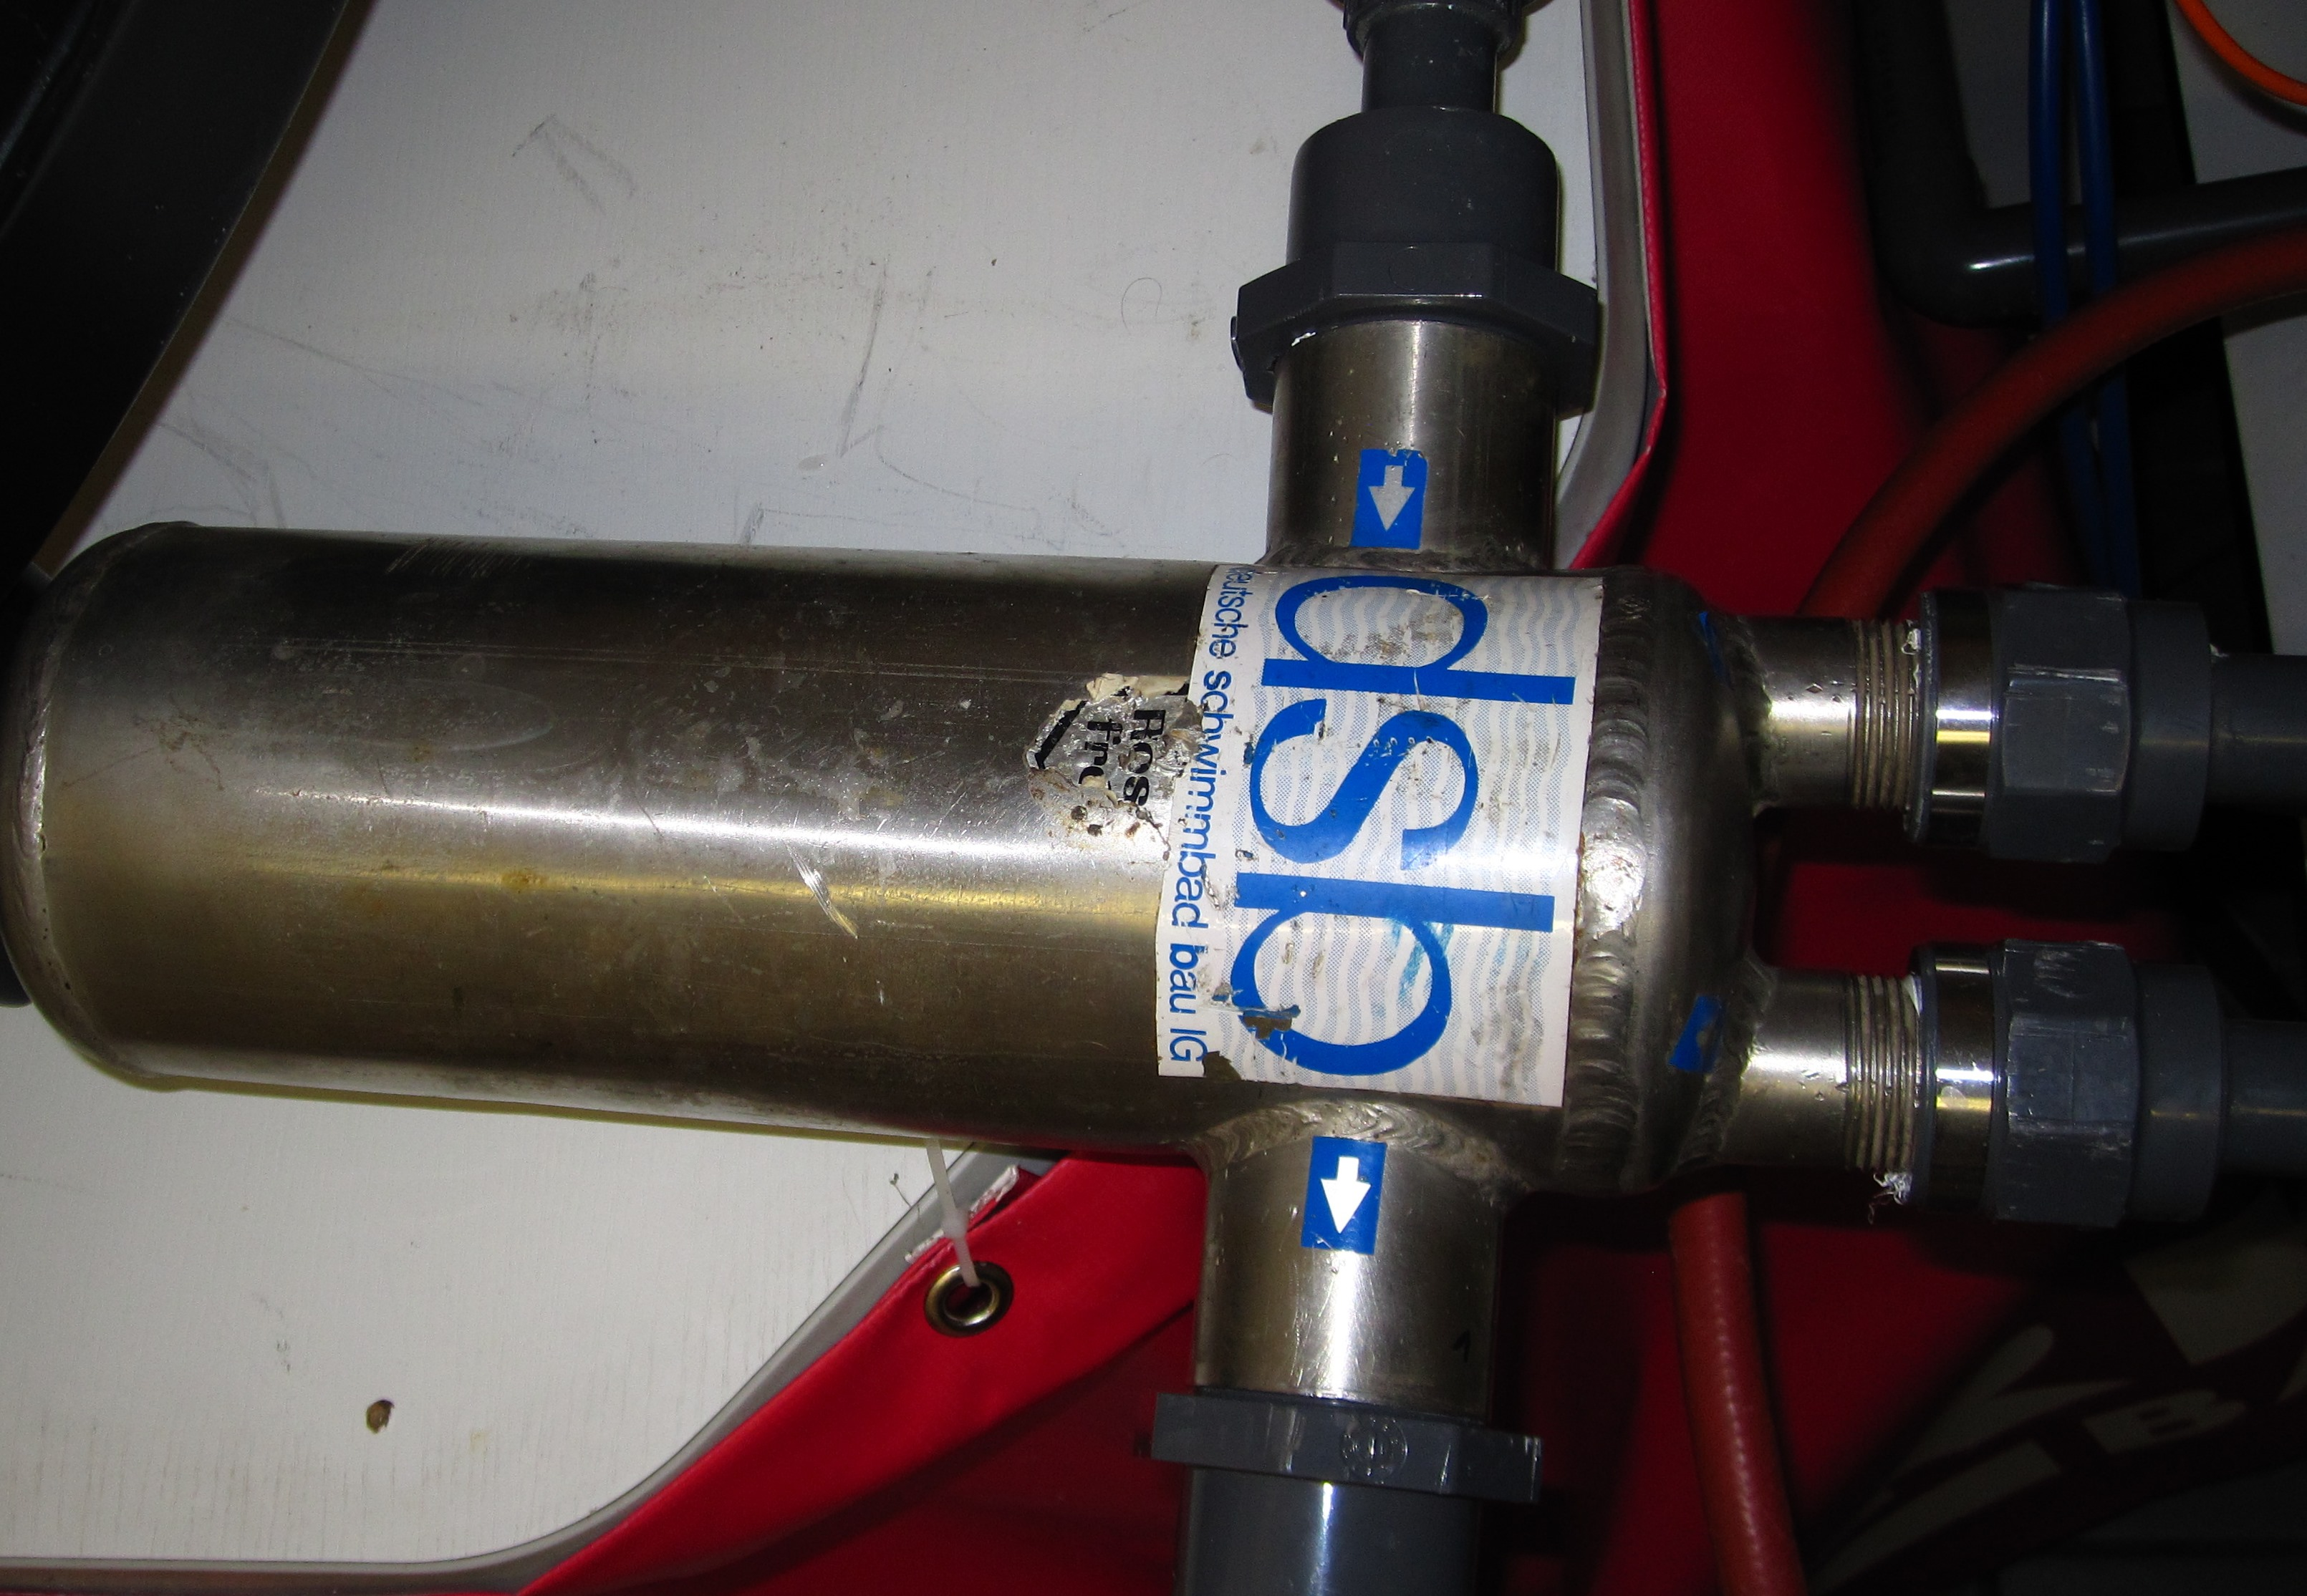
\includegraphics[width=\textwidth]{600-Appendices/Examples/Heat_Exchanger.jpg}}
		\put(4,5){\colorbox{red!20}{\framebox[1.1\width]{Concentrate in}}}
		\put(3,1){\colorbox{red!20}{\framebox[1.1\width]{Concentrate out}}}
		\put(7,4.5){\colorbox{blue!20}{\framebox[1.1\width]{From exchanger}}}
		\put(7,1.5){\colorbox{blue!20}{\framebox[1.1\width]{To exchanger}}}
	\end{picture}              
	\caption{Heat exchanger with flow of media}
	\label{fig:HeatExchanger}
\end{figure}

\paragraph{Demonstration of citation}
Table \ref{tbl:CitationStyles} shows some different options on how to cite a source. The examples are done using natbib package.

\begin{table}
	\begin{center}
		\caption{\label{tbl:CitationStyles}Some styles to citation}
		\begin{tabular}{lll}
			\hline \\
			Command & 	Output	& Description \\
			\\
			\hline \\
			\verb! \cite{ref} ! & \cite{Monippally2010} & Citation\\
			\verb! \textcite[page]{ref} ! & \textcite[p. 20]{Monippally2010} & Textual citation\\
			\verb! \parencite[chapter]{ref} ! & \parencite[chap. 4]{Monippally2010} & Parenthetical citation\\
			
			\verb! \citeauthor{ref} ! & \citeauthor{Monippally2010} & Name of author\\
			\verb! \citeyear{ref} ! & \citeyear{Monippally2010} & Year of publication\\
			\hline \\
		\end{tabular}  
	\end{center}
\end{table}

\cite{HowWriteDissertation} gives some guidance on how to structure a dissertation.

\paragraph{Demonstration of formulas}
Equation \eqref{equ:Population} shows the geometrical projection formula for population growth.
The parameters description is done using the macro \textit{conditions}, defined at NDUmacros.tex.

\begin{figure} % figure is used here to keep the block together
\begin{equation}\label{equ:Population}
P_f=P_0(1+\frac{i}{100})^t
\end{equation}
where:
\begin{conditions}
	P_f	&	Future population \\
	P_0	&	Current population \\
	i	&	Growth rate in \% \\   
	t	&	Time in years
\end{conditions}
\end{figure}

The Hazen-Williams formula expressed in metric units as seen in \eqref{equ:Hazen-William}.
\begin{figure} % figure is used here to keep the block together
\begin{equation}\label{equ:Hazen-William}
H[m]= \Big( \frac{6.78 L}{d^{1.165}} \Big) \Big({\frac{V}{C}} \Big)^{1.85}
\end{equation}
where:
\begin{conditions}
	H	&	Headloss \\
	L	&	Length of pipe\\
	d	&	Internal diameter of pipe \\   
	V	&	Flow \\
	C	&	Coefficient
\end{conditions}
\end{figure}
\paragraph{Demonstration of links}
Use \verb!\href{URL}{DESCRIPTION}! to add a link with description.
Use \verb!\url{URL}! to add a link without a description.

The Water Research \& Development Centre's website: \url{https://nduwrdc.org}

\paragraph{Demonstration of symbols}
In TeXstudio instead of viewing the \textit{Structure} in the side panel, click on $\ast$ to get a list of symbols. Once inserted a leading and trailing \$ must be placed around the symbol code. Some examples displayed using tabbing:
\begin{tabbing}
	\hspace{2in}     			\= \hspace{0.40in}  \= \hspace{1in}    		\kill
	\verb!$\pm$! 				\> $\rightarrow$ 	\> $\pm$ 				\\
	\verb!$\Longrightarrow$! 	\> $\rightarrow$ 	\> $\Longrightarrow$ 	\\
	\verb!$\alpha$! 			\> $\rightarrow$ 	\> $\alpha$ 			\\
	\verb!$\pi$! 				\> $\rightarrow$ 	\> $\pi$ 				\\
	\verb!$\mu$! 				\> $\rightarrow$ 	\> $\mu$	 			\\
\end{tabbing}

\paragraph{Demonstration of a flowchart}
You can follow the instructions of overleaf.com on creating flowcharts,  \url{https://www.overleaf.com/learn/latex/LaTeX\_Graphics\_using\_TikZ:\_A\_Tutorial\_for\_Beginners\_(Part\_3)\%E2\%80\%94Creating\_Flowcharts}, to achieve figures~\ref{fig:flowchart1}~and~\ref{fig:flowchart2}.
\begin{figure}
	\centering
	\begin{tikzpicture}[node distance=2cm]
		\node (start) [startstop] {Something to start with};
		\node (proc1) [process, right of=start, xshift=4cm] {Something else};
		\node (proc2) [process, below of=proc1, yshift=-0.5cm] {
			\begin{minipage}{4cm} %use minipage to have lists
				\begin{itemize}
					\item first item
					\item second item
				\end{itemize}
			\end{minipage}
			};
		\node (proc3) [process, below of=start, yshift=-.5cm] {more here};
		\node (proc4) [process, below of=proc3, xshift=2.5cm, yshift=-0.5cm,  align=left] {many lines\\line 2\\line 3\\line 4}; % align-key needed for \\linebreak 
		\draw [arrow] (start) -- (proc1);
		\draw [arrow] (start) -- (proc3);
		\draw [arrow] (proc1) -- (proc2);
		\draw [arrow] (proc3) -- (proc4);
		\draw [arrow] (proc4) -- (proc2);
	\end{tikzpicture}	
	\caption{Example of a flow chart}
	\label{fig:flowchart1}
\end{figure}

\begin{figure}
	\centering
	\begin{tikzpicture}[node distance=4cm]
		\node (start) [startstop] {Something to start with};
		\node (proc1) [process, right of=start, xshift=0.5cm, yshift=2cm] {A};
		\node (proc2) [process, right of=start, xshift=0.5cm, yshift=-2cm] {B};
		\node (proc3) [process, right of=proc1, yshift=1cm, align=left] {A1\\A1a};
		\node (proc4) [process, right of=proc1, yshift=-1cm, align=left] {A2\\A2b};
		\node (proc5) [process, right of=proc2, yshift=1cm] {B1};
		\node (proc6) [process, right of=proc2, yshift=-1cm] {B2};
		\draw [arrow] (start) -- (proc1);
		\draw [arrow] (start) -- (proc2);
		\draw [arrow] (proc1) -- (proc3);
		\draw [arrow] (proc1) -- (proc4);
		\draw [arrow] (proc2) -- (proc5);
		\draw [arrow] (proc2) -- (proc6);
	\end{tikzpicture}	
	\caption{Some sort of a tree}
	\label{fig:flowchart2}
\end{figure}

\paragraph{Demonstration of a circular diagram}
There is a number of examples using the smartdiagram package here: \url{https://texample.net/tikz/examples/all/}. Figure~\ref{fig:flowchart3} is one of them.
\begin{figure}
	\centering
	\smartdiagram[circular diagram:clockwise]{ABC, DEF, GHI, JKL, MNO}
	\caption{Circular diagram}
	\label{fig:flowchart3}
\end{figure}
